% Author: Izaak Neutelings (October 2021)
% Inspiration
%   "Very special relativity - An illustrated guide", Sander Bais (2007)
%   http://people.uncw.edu/hermanr/GR/Minkowski/Minkowski.pdf
\documentclass[border=3pt,tikz]{standalone}
\usepackage{amsmath} % for \text
\usepackage{etoolbox} % ifthen
\usepackage[outline]{contour} % glow around text
\usetikzlibrary{calc} % for adding up coordinates
\usetikzlibrary{decorations.markings,decorations.pathmorphing}
\usetikzlibrary{angles,quotes} % for pic (angle labels)
\usetikzlibrary{arrows.meta} % for arrow size
\usepackage{xfp} % higher precision (16 digits?)
\contourlength{1.1pt}

\tikzset{>=latex} % for LaTeX arrow head
\colorlet{myred}{red!85!black}
\colorlet{mydarkred}{red!55!black}
\colorlet{mylightred}{red!85!black!12}
\colorlet{myfieldred}{mydarkred!5} % for S' background
\colorlet{myredhighlight}{myred!20} % highlights simultaneity in ladder paradox
\colorlet{myblue}{blue!80!black}
\colorlet{mydarkblue}{blue!50!black}
\colorlet{mylightblue}{blue!50!black!30}
\colorlet{mylightblue2}{myblue!10}
\colorlet{mygreen}{green!80!black}
\colorlet{mypurple}{blue!40!red!80!black}
\colorlet{mydarkgreen}{green!50!black}
\colorlet{mydarkpurple}{blue!40!red!50!black}
\colorlet{myorange}{orange!40!yellow!95!black}
\colorlet{mydarkorange}{orange!40!yellow!85!black}
\colorlet{mybrown}{brown!20!orange!90!black}
\colorlet{mydarkbrown}{brown!20!orange!55!black}
\colorlet{mypurplehighlight}{mydarkpurple!20} % highlights simultaneity in ladder paradox
\tikzstyle{world line}=[myblue!40,line width=0.3]
\tikzstyle{world line t}=[mypurple!50!myblue!40,line width=0.3]
\tikzstyle{world line'}=[mydarkred!40,line width=0.3]
\tikzstyle{mysmallarr}=[-{Latex[length=3,width=2]},thin]
\tikzstyle{mydashed}=[dash pattern=on 3 off 3]
\tikzstyle{rod}=[mydarkbrown,draw=mydarkbrown,double=mybrown,double distance=2pt,
                 line width=0.2,line cap=round,shorten >=1pt,shorten <=1pt]
%\tikzstyle{rod'}=[rod,draw=mydarkbrown!80!red!85,double=mybrown!80!red!85]
\tikzstyle{vector}=[->,line width=1,line cap=round]
\tikzstyle{vector'}=[vector,shorten >=1.2]
\tikzstyle{particle}=[mygreen,line width=0.9]
\tikzstyle{photon}=[-{Latex[length=5,width=4]},myorange,line width=0.8,decorate,
                    decoration={snake,amplitude=1.0,segment length=5,post length=5}]

\def\tick#1#2{\draw[thick] (#1) ++ (#2:0.06) --++ (#2-180:0.12)}
\def\tickp#1#2{\draw[thick,mydarkred] (#1) ++ (#2:0.06) --++ (#2-180:0.12)}
\def\Nsamples{100} % number samples in plot

\begin{document}

% SPACETIME DIAGRAM - EUCLIDEAN ROTATION
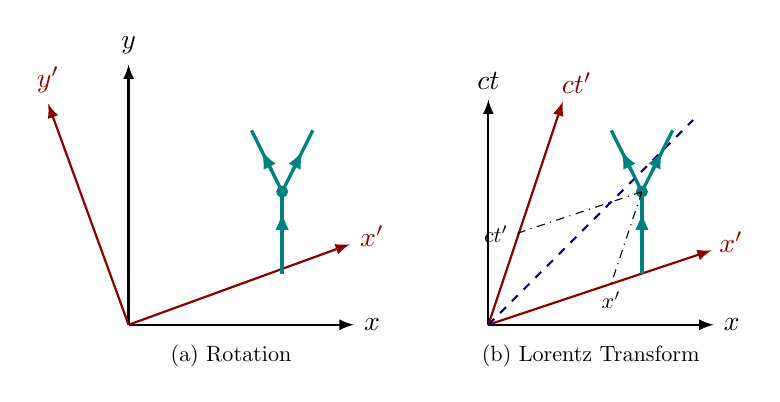
\begin{tikzpicture}[scale=1.3]
  \begin{scope}
  
    \def\xmax{2}
    \def\xmaxp{2.1} % maximum of rotated axis
    \def\Nlines{5} % number of world lines (at constant x/t)
    \pgfmathsetmacro\ang{20} % angle between x and x' axes
    \pgfmathsetmacro\d{0.9*\xmax/\Nlines} % grid size
    \coordinate (O) at (0,0);
    \coordinate (X) at (\xmax+0.2,0);
    \coordinate (T) at (0,{(1+0.5*sin(\ang))*\xmax+0.2});
    \coordinate (X') at (\ang:\xmaxp+0.2);
    \coordinate (T') at (90+\ang:\xmaxp+0.2);
    
    % AXES
    \draw[->,thick] (0,0) -- (T) node[above] {$y$};
    \draw[->,thick] (0,0) -- (X) node[right] {$x$};
    \draw[->,thick,mydarkred] (90+\ang:0) -- (T')
        node[above] {$y'$};
    \draw[->,thick,mydarkred] (\ang:0) -- (X')
        node[above=3,right=0] {$x'$};
    
     % EVENT

    \draw[->, very thick, teal] (1.5, 0.5) -- (1.5, 1.1);
    \draw[, very thick, teal] (1.5, 0.8) -- (1.5, 1.3);
    \draw[color=teal, fill=teal] (1.5, 1.3) circle (1.5pt);
    \draw[->, very thick, teal] (1.5, 1.3) -- (1.3, 1.7);
    \draw[ very thick, teal] (1.4, 1.5) -- (1.2, 1.9);
    \draw[->, very thick, teal] (1.5, 1.3) -- (1.7, 1.7);
    \draw[ very thick, teal] (1.6, 1.5) -- (1.8, 1.9);
    \node[scale = 0.8] at (1, -0.3) {(a) Rotation};
  \end{scope}

  \begin{scope}[xshift=100]
    \def\xmax{2}
    \def\xmaxp{2.1} % maximum of rotated axis
    \def\Nlines{5} % number of world lines (at constant x/t)
    \pgfmathsetmacro\ang{atan(1/3)} % angle between x and x' axes
    \pgfmathsetmacro\d{0.9*\xmax/\Nlines} % grid size
    \pgfmathsetmacro\D{\d/cos(\ang)/sqrt(1-tan(\ang)^2)} % grid size, boosted
    \coordinate (O) at (0,0);
    \coordinate (X) at (\xmax+0.2,0);
    \coordinate (T) at (0,\xmax+0.2);
    \coordinate (X') at (\ang:\xmaxp+0.2);
    \coordinate (T') at (90-\ang:\xmaxp+0.2);
    
 
    % AXES
    \draw[->,thick] (0,0) -- (T) node[above] {$ct$};
    \draw[->,thick] (0,0) -- (X) node[right] {$x$};
    \draw[->,thick,mydarkred] (90-\ang:0) -- (T')
        node[right=5,above=-1] {$ct'$};
    \draw[->,thick,mydarkred] (\ang:0) -- (X') node[above=3, right=-1] {$x'$};
    
    % Light Line
    \draw[,thick, dashed, mydarkblue] (0, 0) -- (2, 2);

     % EVENT

    \draw[->, very thick, teal] (1.5, 0.5) -- (1.5, 1.1);
    \draw[, very thick, teal] (1.5, 0.8) -- (1.5, 1.3);
    \draw[color=teal, fill=teal] (1.5, 1.3) circle (1.5pt);
    \draw[->, very thick, teal] (1.5, 1.3) -- (1.3, 1.7);
    \draw[ very thick, teal] (1.4, 1.5) -- (1.2, 1.9);
    \draw[->, very thick, teal] (1.5, 1.3) -- (1.7, 1.7);
    \draw[ very thick, teal] (1.6, 1.5) -- (1.8, 1.9);

    \draw[dashdotted] (1.5, 1.3) -- ++(180+\ang:1.3) node [left, scale=0.8] {$ct'$};
    \draw[dashdotted] (1.5, 1.3) -- ++(270-\ang:0.95) node [below, scale=0.8] {$x'$};
    \node[scale = 0.8] at (1, -0.3) {(b) Lorentz Transform};
  \end{scope}
    
\end{tikzpicture}


\end{document}